\chapter{Einführung und Aufbau}
\label{cha:Einführung}

Object detection is a technology related to computer vision and image processing that deals with detecting instances of objects of a certain class (such as humans, cars, animals and drones) in digital images and videos. It has roots dating back to 1990s, although there has been major leaps in techniques and algorithms over the years. In the relatively recent years, deep learning methods have been prevalent in the object detection technologies.

In the rapidly advancing field of cameras and computer vision, the development of robust object recognition models is essential for applications ranging from autonomous systems to surveillance and beyond in many different fields. As technology continues to evolve, the integration of different forms of imaging has become a key focus to enhance the adaptability and reliability of these models. Visible images are affected by environmental and illumination variations such as low lighting and sun glare; meanwhile thermal and infrared images are noisy and have low resolution. \cite[p.1]{systematicreview23} The main advantage of thermal and infrared imagery is that they are not affected by light conditions, thus they can see objects that would otherwise be very difficult or even impossible to see with visible imagery.

The increasing usage and market size of infrared cameras and imagery (see Figure \ref{fig:marketsize}) and AI-based object detection continuously require better optimized and well performing models, especially in difficult environmental conditions such as rainy, foggy weather and high or low temperatures. Improvements to these detection methods and systems can have benefits extending into fields such as autonomous vehicles, agriculture, smart cities, search and rescue operations, public safety, security and military. 

\begin{figure}[!ht]
	\centering
		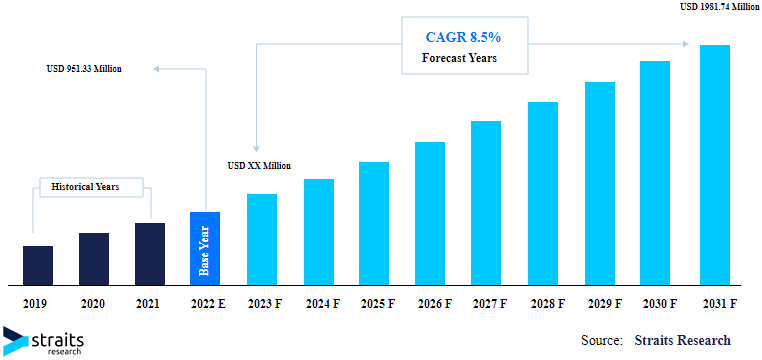
\includegraphics[width=0.75\textwidth]{images/straitsresearch_infrared_camera_marketsize.png}
	\caption{Infrared Camera Market Size \citep{infraredcameramarket}}
	\label{fig:marketsize}
\end{figure}

Object detection in the visible spectrum is has seen a lot of interest and progress throughout the history of object detection. Deep learning methods have been developed within the past decade, that have continued to bring faster and more accurate detection performances. Some of the most prominent methods and algorithms currently used in object detection can be named as; R-CNN \citep{girshick2014rcnn} and it's variants such as Fast R-CNN \citep{girshick2015fast} and Faster R-CNN \citep{ren2015faster}, You Only Look Once(YOLO) \citep{redmon2016look}, Single Shot Multibox Detector(SSD) \citep{Liu_2016ssd}, RetinaNet \citep{lin2018focal}, EfficientDet \citep{tan2020efficientdet}.

The IR spectrum, on the other hand, is a relatively newer field in the context of object detection. Though it has been explored a lot, there really is no limit to the performance that may be achieved with further development. There has been works so far that have attempted to utilise the fusion of IR-RGB images to achieve better detection performances such as \cite{rgb-infrared2022}


%TODO add "aufbau" part that explains the structure of the paper





